\chapter{Baggrund}
\section{Hjertet \& Kredsløb}
Hjertet, \textit{cor}, er en hul muskel, der har til opgave at pumpe blodet rundt til hele kroppen. Hjertet består af i alt fire kamre, som det kan ses på figur 3.1 nedenfor. To forkamre, atrier, og to hjertekamre, ventrikler. Atrierne fungere primært som reservoir for blod, mens ventriklerne fungerer som den effektive pumpe.\\

\begin{figure}[htb]
	\centering
	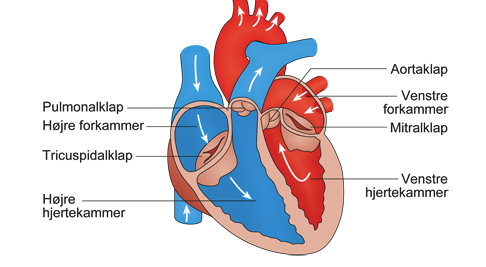
\includegraphics[width=1\textwidth]{Figurer/Fysio/Hjertet}
	\caption{Hjerte med forklarende pile \protect\footnotemark} 
\end{figure}
\footnotetext{http://www.hjertelunge.dk/hjertesygdomme/hjerte\_og\_kredsloeb/hjertet/}

Hjertekamrene og forkamrene er adskilt fra hinanden af anulus fibrosus, som er en plade af bindevæv. Anulus fibrosus består af fire bindevævsringe, der er forbundet med hinanden. To af disse udgør åbningerne mellem atrierne og ventriklerne. De to sidste danner åbningerne mellem højre hjertekammer og lungepulsåren og venstre ventrikel og hovedpulsåren. Ved alle bindevævsringene er der klapper, der fungere som ventiler.\\ 
AV-klapperne sidder mellem atrierne og ventriklerne. Klappen mellem højre atrium og ventrikel kaldes tricuspidalklap, mens klappen mellem venstre atrium og ventrikel kaldes mitralklap, se figur 3.1. Aortaklappen er placeret ved afgangen af hovedpulsåren og pulmonalklappen ved afgangen af lungepulsåren. Klapperne fungere således, at blodet kun kan løbe én vej gennem dem. Åbningen samt lukningen af disse er en passiv proces, som bestemmes af forskelle i væsketrykket på de to sider af klapperne.\\ 

\begin{figure}[htb]
	\centering
	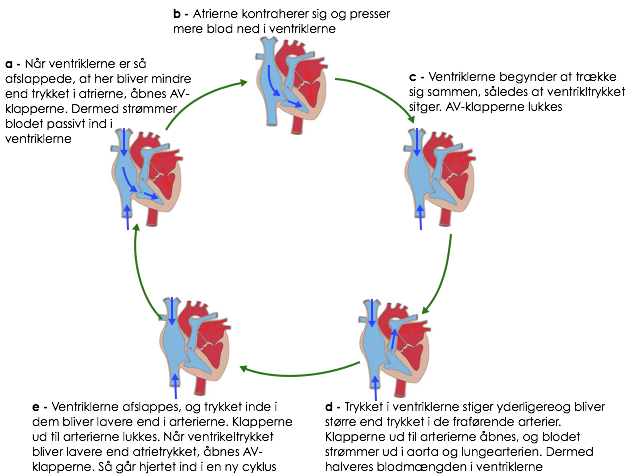
\includegraphics[width=1\textwidth]{Figurer/Fysio/Cyklus}
	\caption{De forskellige faser i hjertets cyklus \protect\footnotemark}
\end{figure}
\footnotetext{Billede fra "Menneskets anatomi og fysiologi" s. 273 figur 9.6}

Hjertets cyklus, som er illustreret ved figur 3.2, inddeles i to hovedfaser. Den første kaldes diastolen. I diastolen er ventriklerne afslappede og fyldes med blod. Det vil sige, at trykket i ventriklerne bliver lavere end trykket i atrierne, således at AV-klapperne åbnes, og blodet begynder at strømme ind i ventriklerne. Under hele diastolen er aortaklappen lukket. Den anden fase kaldes systolen. I systolen kontraherer ventriklerne sig. Trykket i ventriklerne overstiger trykket i atrierne således, at AV-klapperne lukkes, så tilbagestrømning af blod til atrierne forhindres. Når ventriklerne har kontraheret sig så meget, at trykket i ventriklerne overstiger trykket i hovedpulsåren samt i lungepulsåren, åbnes aortaklappen og pulmonalklappen, og blodet strømmer ud i hovedpulsåren og lungepulsåren. Ventriklernes tryk falder igen til under atriernes tryk, hvilket påvirker, at AV-klapperne åbnes igen og hjertets cyklus starter forfra.\\

\section{Hæmodynamik}
Når blodet skal fra hjertet og rundt kroppen taler man om et blodflow. Blodets flow opfører sig som shear thinning fluid, som gør sig gældende ved ikke-newtonske væsker med formindsket viskositet. At blodet hører under denne kategori, skyldes at erythrocytterne (de røde blodlegemer) organiseres ved et øget flow. \\
Når hjertet pumper opstår der et tryk i blodkarrene. Blodtrykket er resultatet af hjertets pumpearbejde og modstanden mod blodstrømmen i blodkredsløbet. Trykket er højest i arterierne, der forlader hjertet og trykket er lavest i venerne, der fører tilbage til hjertet.\footnote{\url{http://www.denstoredanske.dk/Krop,_psyke_og_sundhed/Sundhedsvidenskab/Fysiologi/blodtryk}}\\
Blodtrykket deles op i et systolisk tryk og et diastolisk tryk. Det systolsike tryk er det tryk, der opstår under hjertets sammentrækning, altså hjertets uddrivningsfase. Det diasoliske tryk opsår i hjertets afslapningsfase. I disse faser er det arterielle blodflow ikke steady med derimod pulsatilt. \\Dog falder trykket ikke til 0 i diastolen pga. pulsårevæggenes elasticitet. Forholdet mellem tryk og volumen er illustreret i figur \ref{tryk og volumen}
\begin{figure}[H]
	\centering
	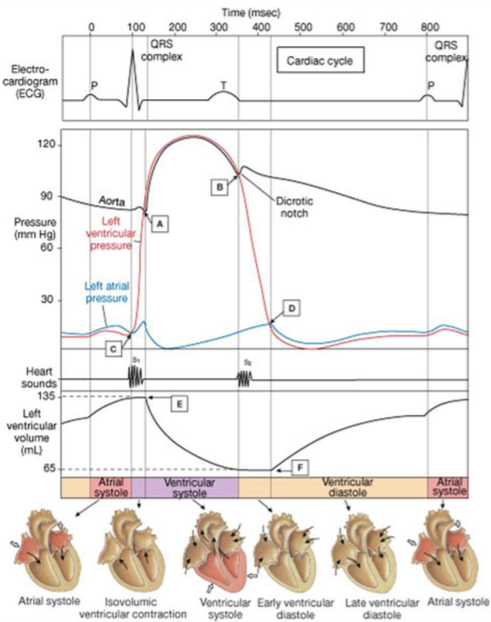
\includegraphics[width=0.8\textwidth]{Figurer/Fysio/TrykOgVolumen}
	\caption{Forhold mellem tryk og volumen}
	\label{tryk og volumen}
\end{figure}
Figur \ref{tryk og volumen} viser yderligere også hvordan hjerteklappens lukning fungerer når et trykfald herover ændrer retning. I det systemiske kredsløb er første kar aorta, som grundet sin elasticitet vil få hovedparten af blodmængden, pumpet ud af venstre ventrikel, til at blive opstemt i aorta. Dette medfører at der oplagres en elastisk potentiel energi i aortavæggen. Denne energi udgør et tryk, der har indflydelse på og bidrager til, et blodflow i diastolen efter aortaklappens lukning og hjertets uddrivningsfase. 

\section{Hypertension}
Hypertension defineres ud fra vedtagne blodtryksgrænser. De nuværende blodtryksgrænser ligger på et systolisk tryk over 140mmHg og/eller et diastolisk tryk på over 90mmHg. Disse grænserværdier gælder uanset patientens alder. Grænseværdierne er dog kun et udgangspunkt for der kan godt opstå hypertension hos en person med i forvejen for lavt blodtryk og i dette tilfælde vil grænseværdierne ikke nå op på værdien for definitionen af hypertension.\\
Hypertension medfører betydelig øget risiko for kardiovaskulære sygdomme som oftest er apopleksi og iskæmisk hjertesygdom. Herudover kan hypertension medfører påvirkning af nyrene.
\footnote{\url{https://www.sundhed.dk/sundhedsfaglig/laegehaandbogen/hjerte-kar/tilstande-og-sygdomme/oevrige-sygdomme/hypertension/}} 

\section{Hypotension}
Hypotension defineres som et vedvarende systolsik tryk under 100mmHg i hvile. \\
Under operationer og traumer er hypotension en mere alvorlig ting og defineres ofte som shock.\\
Shock er defineret ved en patofysiologisk tilstand karakteriseret ved, at blodcirkulationen er utilstrækkelig til at imødekomme kroppens metaboliske behov. Blodtryksgrænsen for shock angives forsimplet ofte at være systolisk blodtryk på under 90 eller et fald i systolisk tryk på 40 mmHg.
\footnote{\url{https://www.sundhed.dk/sundhedsfaglig/laegehaandbogen/akut-og-foerstehjaelp/tilstande-og-sygdomme/hjerte-kar/shock/}}

\section{Blodtryksmåling}
For at kunne detektere et blodtryk som beskrevet i ovenstående, er det nødvendigt at foretage en eller anden form for blodtryksmåling. \\
Der findes mange former for blodtryks målinger, de mest hyppigt brugte er dog de non-invasive og invasive målinger. De non-invasive målinger kan være målemetoder som den klassiske blodtryksmåling med manchet, stetoskop og kviksølvsmanometer. Den invasive metode indebærer en indsættelse af instrument i kroppen og benyttes blandt andet på operationsstuer. Et invasiv blodtryksmåling apparat kan deles op i to generelle kategorier. Den meste brugte kliniske metode er metoden er at koble det vaskulære tryk til en ekstern sensor element via et væskefyldt kateter. Den anden metode er en metode, hvor vand koblingen her bliver elimineret ved at inkorporere sensoren i spidsen af kateteret i det vaskulære system.

\section{Sensorer}
En sensor er en transducer, der transformerer en fysisk målestørrelse til elektrisk energi. Til måling af fysiologiske størrelser som blodtryk bruges sensorer som omformer flow til elektrisk energi. Et eksempel på sådanne sensorer er en strain gauge som er en resistiv transducer. Strain gauges klassificeres enten som bundne eller ubundne, hvor den ubundne giver en temperatur kompensation mens den bundne kan have udsving grundet temperaturen.\\
Den ubundne strain gauge består af fire set af stræk følsomme ledninger, der er forbundet så de danner en wheatstone bro, se figur \ref{StrainGauge}. Disse ledninger er monteret under tryk mellem rammen og det bevægelige armatur således den maksimal belastning strain gaugen kan holde til, er større end den forventede udefrakommende komprimerende belastning. Dette er nødvendigt for ikke at skade ledningerne. Disse typer af sensorer kan blive brugt til at konvertere blodtryk til membran bevægelse, videre til modstands ændring og til sidst et elektrisk signal. Bro sammenkoblingen giver en temperatur kompensation og den giver fire gange så stort et output fordi alle fire arme indeholder aktive gages.\\
\begin{figure}[H]
	\centering
	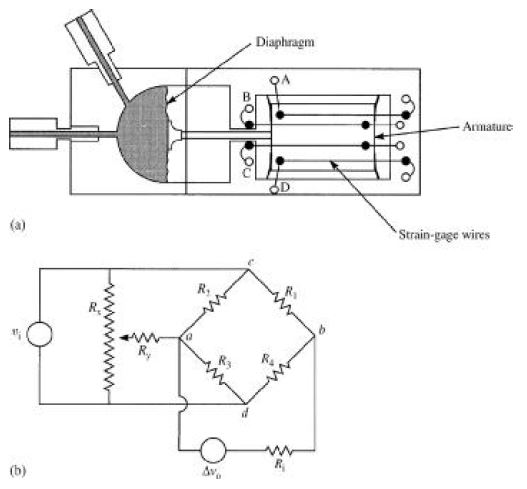
\includegraphics[width=0.6\textwidth]{Figurer/Hardware/straingauge}
	\caption{(a) Ubundet strain gauge tryk sensor. Membranen er direkte koblet via et armaratur til et ubundet strain gauge system. Med stigende tryk, øges strækket over parret B og C, mens strækket over parret A og D sænkes. (b) Wheatstone bro med fire aktive elementer: $R_{1} = B, R_{2} = A, R_{3} = D og R_{4} = C $ når den ubundne strian gauge er forbundet til translationel bevægelse. Resistoren$ R_{y}$ og potentiometret $R_{x}$ bruges til at balancere broen, $V_{i}$ er den tilførte spænding og $\Delta v_{0}$ er output spænding på et voltmeter eller lignende apparat med en indre modstand på $R_{i}$. Kilde: Webster - Medical instrumentation, application and design 4th Edition}
	\label{StrainGauge}
\end{figure}






\section{Programmerings teori}
Helt generelt er softwaren i blodtrykssystemet bygget op omkring 3-lagsmodellen. 3-lagsmodellen er bestående af lagene præsentationslag, logiklag og datalag. \textbf{Skriv mere!}
\subsection{Tråde}
Tråd programmering benyttes, når man som her ønsker flere opgaver i programmet udført løbende. Dette kan gør sig gældende eksempelvis ved at programmet ønsker at indlæse data og vise det i en graf, samtidig med at brugeren har adgang til alle interfacets funktioner. Det er disse delprocesser, som udgøre trådene. Hvis en enkelt tråd skulle gå i stå, skal de andre tråde stadig køre, således at programmet stadig kører videre. 
\subsection{Observer}
\subsection{Push pull}

